%%%
 %
 % Copyright (C) 2019 Ángel Iván Gladín García
 %
 % This program is free software: you can redistribute it and/or modify
 % it under the terms of the GNU General Public License as published by
 % the Free Software Foundation, either version 3 of the License, or
 % (at your option) any later version.
 %
 % This program is distributed in the hope that it will be useful,
 % but WITHOUT ANY WARRANTY; without even the implied warranty of
 % MERCHANTABILITY or FITNESS FOR A PARTICULAR PURPOSE.  See the
 % GNU General Public License for more details.
 %
 % You should have received a copy of the GNU General Public License
 % along with this program.  If not, see <http://www.gnu.org/licenses/>.
%%%

%%%%%%%%%%%%%%%%%%%%%%%%%%%%%%%%%%%%%%%%%%%%%%%%%%%%%%%%%%%%%%%%%%%%%%%%%%%%%%%%%%%%%%%%%
\documentclass[11pt,letterpaper]{report}
\usepackage[margin=0.5in]{geometry}
\usepackage[utf8]{inputenc}
\usepackage[spanish]{babel}
\decimalpoint

\usepackage{listings}
\usepackage{color}
\usepackage{graphicx}
\usepackage{enumerate}
\usepackage{enumitem}
\usepackage{float}

\usepackage{longtable}
\usepackage{hyperref}
\usepackage{commath}

\usepackage{bbm}
\usepackage{dsfont}
\usepackage{mathrsfs}
\usepackage{amsmath,amsthm,amssymb}
\usepackage{mathtools}
\usepackage{longtable}
%%%%%%%%%%%%%%%%%%%%%%%%%%%%%%%%%%%%%%%%%%%%%%%%%%%%%%%%%%%%%%%%%%%%%%%%%%%%%%%%%%%%%%%%%%%%%%%%5

\usepackage{import}

\usepackage[utf8]{inputenc}

\usepackage{listings}
\usepackage{color}

\definecolor{codegreen}{rgb}{0,0.6,0}
\definecolor{codegray}{rgb}{0.5,0.5,0.5}
\definecolor{codepurple}{rgb}{0.58,0,0.82}
\definecolor{backcolour}{rgb}{0.95,0.95,0.92}

\lstdefinestyle{mystyle}{
    backgroundcolor=\color{backcolour},   
    commentstyle=\color{codegreen},
    keywordstyle=\color{magenta},
    numberstyle=\tiny\color{codegray},
    stringstyle=\color{codepurple},
    basicstyle=\footnotesize,
    breakatwhitespace=false,         
    breaklines=true,                 
    captionpos=b,                    
    keepspaces=true,                 
    numbers=left,                    
    numbersep=5pt,                  
    showspaces=false,                
    showstringspaces=false,
    showtabs=false,                  
    tabsize=2
}

\lstset{style=mystyle}
%%%%%%%%%%%%%%%%%%%%%%%%%%%%%%%%%%%%%%%%%%%%%%%%%%%%%%%%%%%%%%%%%%%%%%%%%%%%%%%%%%%%%%%%%


%%%%%%%%%%%%%%%%%%%%%%%%%%%%%%%%%%%%%%%%%%%%%%%%%%%%%%%%%%%%%%%%%%%%%%%%%%%%%%%%%%%%%%%%%
\newcommand{\Z}{\mathbb{Z}}
\newcommand{\N}{\mathbb{N}}
\newcommand{\Q}{\mathbb{Q}}
\newcommand{\R}{\mathbb{R}}
\newcommand{\Oh}{\mathcal{O}} %% Notacion "O"
\newcommand{\lra}{\longrightarrow}
\newcommand{\ra}{\rightarrow}
\newcommand{\ord}{\text{ord}}
\newcommand{\sol}{\textbf{\underline{Solución}: }} %% Solucion

%%%%%%%%%%%%%%%%%%%%%%%%%%%%%%%%%%%%%%%%%%%%%%%%%%%%%%%%%%%%%%%%%%%%%%%%%%%%%%%%%%%%%%%%%

\begin{document}

%%%%%%%%%%%%%%%%%%%%%%%%%%%%%%%%%%%%%%%%%%%%%%%%%%%%%%%%%%%%%%%%%%%%%%%%%%%%%%%%%%%%%%%%%
\title{
        Universidad Nacional Autónoma de México\\
        Facultad de Ciencias\\
        Probabilidad I\\
    \vspace{1cm}
    \large
        \textbf{Tarea 2}\\
        \textbf{Propiedades Básicas de la Probabilidad}
}
\author{
    Ángel Iván Gladín García\\
    No. cuenta: 313112470\\
    \texttt{angelgladin@ciencias.unam.mx}
    \and
    Mario Navarrete Baltazar\\
    No. cuenta: 315218413\\
    \texttt{qwertyuiop@ciencias.unam.mx}
}
\date{13 de Septiembre 2019}
\maketitle
%%%%%%%%%%%%%%%%%%%%%%%%%%%%%%%%%%%%%%%%%%%%%%%%%%%%%%%%%%%%%%%%%%%%%%%%%%%%%%%%%%%%%%%%%

%%%%%%%%%%%%%%%%%%%%%%%%%%%%%%%%%%%%%%%%%%%%%%%%%%%%%%%%%%%%%%%%%%%%%%%%%%%%%%%%%%%%%%%%%
\newtheorem{theorem}{Teorema}
\newtheorem{example}{Ejemplo}
\newtheorem{corollary}{Corolario}
\newtheorem{lemma}{Lemma}
\newtheorem{definition}{Definicion}
\newtheorem{prop}{Proposicion}
%%%%%%%%%%%%%%%%%%%%%%%%%%%%%%%%%%%%%%%%%%%%%%%%%%%%%%%%%%%%%%%%%%%%%%%%%%%%%%%%%%%%%%%%%

%%%%%%%%%%%%%%%%%%%%%%%%%%%%%%%%%%%%%%%%%%%%%%%%%%%%%%%%%%%%%%%%%%%%%%%%%%%%%%%%%%%%%%%%%
\begin{enumerate}

\item Imaginemos el siguiente experimento aleatorio. ``Se Lanza un dado continuamente hasta que
caiga un 6 y en ese momento dejamos de lanzar el dado''.

\begin{itemize}
    \item Describe el Espacio Muestral asociado a este Experimento Aleatorio

    \sol El espacio muestral es: $S = (x_1,...,x_i)$ con $i \geq 1$, $x_i \not= 6$, con
    $i$ que significa que hasta ese momento salió un 6.

    \item Sea $E_n$ el evento que denota: El número de lanzamientos necesarios hasta completar el
    experimento. ¿Cuáles puntos del espacio muestral están contenidos en $E_n$?
    
    \sol Las veces que han tirado un dado y no ha salido un 6.

    \item ¿Qué representa $(\cup_{n=1}^{\infty} E_n)^c$ en términos del experimento aleatorio?
    
    \sol Representa el evento en el cual el 6 nunca aparece.    
    
\end{itemize}

\item Tres individuos $A$, $B$ , $C$ se turnan para lanzar una moneda. Al primero que le salga
``Águila'' gana. El espacio muestral asociado a este experimento puede ser definido como:
\[
    S =
    \begin{cases}
        1, 01, 001, 0001, \ldots,\\
        0000\ldots
    \end{cases}
\]

\begin{itemize}
    \item Interpreta el Espacio Muestral
    
    \sol En este experimento los individuos $A$, $B$ , $C$ se turnan para tirar una modena y gana
    el primero que obtenga una ``águila''. En este espacio el \texttt{0} está denotado que salió
    ``sol'' y el \texttt{1} se denota que salió águila. Viendo los casos de $S$; en el
    primero podemos ver los 0's (si hay) precedidos del 1 como cuantas veces (denotado por el
    número de 0's) se tiraron soles hasta que se obtuvo una águila. En el segundo caso dondee es
    una cadena de 0's significa que nunca se obtuvo águila.

    \item Define los siguientes eventos en terminos de $S$.
    
    Asume que $A$ lanza primero la moneda, denoganar lanza $B$, de no ganarlanza $C$ y en
    caso de no ganar nadie se repite el proceso.    

    \sol (Asumiendo que $A$ tiró, luego $B$ y al final $C$ y así consecutivamente.)

    \begin{enumerate}[label=\alph*)]
        \item $A$ gana = $A$
        
        $A$ gana si y solo si hay $3n$ 0's precedidos de él (un \texttt{1}),
        ósea $\underbrace{0 \cdots 0}_{3n} 1$ con $n \in \N$.

        \item $B$ gana = $B$
        
        $B$ gana si y solo si hay $3n+1$ 0's precedidos de él (un \texttt{1}),
        ósea $\underbrace{0 \cdots 0}_{3n+1} 1$ con $n \in \N$.

        \item $(A \cup B)^c$
        
        Este evento significa que $C$ ganó o nadie ganó. Para definir el evento en el que $C$ ganó
        sería análogo a los incisos anteriores, ósea $\underbrace{0 \cdots 0}_{3n+2} 1$, y para
        definir que nadie ganó sería $000\cdots$.
        
    \end{enumerate}

\end{itemize}

\item Si al jugar \textbf{Poker} asumimos que las $\binom{52}{2}$ manos son igualmente probables.
¿Cuál es la probabilidad de que nos hayan repartido:

\begin{itemize}
    \item una Flor? \textbf{Decimos que una mano de poker es una flor si las 5 cartas de la mano son
    del mismo palo}

    \sol $\frac{{4} \cdot \binom{13}{5}}{\binom{52}{5}}$
    

    \item un Par?
    
    \sol $\frac{{13} \binom{4}{2} \binom{12}{3} \binom{4}{1} \binom{4}{1} \binom {4}{1}}{\binom{52}{5}}$


    \item dos Pares?
    
    \sol $\frac{\binom{13}{2}  \binom{4}{2} \binom{4}{2}  \binom {44}{1}}{\binom{52}{5}}$
    

    \item una Tercia?
    
    \sol $\frac{{13}  \binom{4}{3} \binom{12}{2} \binom{4}{1} \binom{4}{1}}{\binom{52}{5}}$


    \item un Poker? \textbf{Tenemos un Poker cuando la mano que nos tocaron contiene 4 cartas con la
    misma denominación y de diferente palo}

    \sol $\frac{{13}  \binom{4}{4} \binom{48}{1}}{\binom{52}{5}}$
    
\end{itemize}

\item Los coeficientes de la ecuación cuadrática $x^2 + bx + c$ están determinados al lanzar un par
de dados, el resultado del primer dado determina el valor de $b$ y el del segundo dado el valor de
$c$. Obtén la probabilidad de que la ecuación tenga soluciones reales.

\sol Como cada dado en cada una de sus caras tiene valores del 1 al 6, y el valor de $b$ está
determinado por el valor del dado y lo mismo para $c$, entonces se tiene que $|\Omega|=36$.
Por otro lado, la ecuación tiene raíces reales si y solo si $b^2 - 4c \geq 0$, entonces los valores
$(b,c)$ que satisfacen esa condición son 
\begin{multline*}
    (2,1),(3,1),(3,2),(4,1),(4,2),(4,3),(4,4),(5,1)(5,2),(5,3),(5,4),\\
    (5,5),(5,6),(6,1),(6,2),(6,3),(6,4),(6,5),(6,6)
\end{multline*}
siendo 19 parejas. Ergo la probabilidad es $\frac{19}{36}$.

\item Dos números $m$ y $n$ son llamados ``primos relativos'' si el 1 es el único divisor común
positivo entre ambos. Así por ejemplo el 8 y el 5 son primos relativos, mientras el 8 y 6 no lo son.
Si un nuúmero es seleccionado al azar del conjunto $\{ 1, 2, 3,\ldots, 63 \}$ . Obtén la
probabilidad de que este número sea primo relativo con el 63.

%% YO NO HICE ESTA Y NI LA LEÍ, POTENCIALMENTE EL QUE LA HIZO LA HIZO MAL.
\sol Los unicos divisores primos de 63 son 3 y 7. Entonces, el numero seleccionado es primero
relativo a 63 si y solo si no es divisible por 3 o 7.

Sean los eventos.

A := {El resultado es divisible entre 3}

B := {El resultado es divisible entre 7}

AB := {El resultado es divisible entre 3 y 7}

Entonces,
A=$\left\lbrace 3,6,9,12,15,18,21,24,27,30,33,36,39,42,45,48,51,54,57,60,63\right\rbrace = 21$ numeros

B=$\left\lbrace 7, 14, 21, 28, 35, 42, 49, 56, 63 \right\rbrace = 9$ numeros 

y AB =$\left\lbrace 21, 42, 63 \right\rbrace = 3 $ numeros 

Por lo tanto, $P(A) = 21/63$, $P(B) = 9/63$ y $P(AB) = \frac{3}{63}$.

Para encontrar la probabilidad de que un numero es primo relativo a 63, tenemos que encontrar la probabilidad que un numero no es disible por 3 esto es $P(AB)^c$

En general,
$P(A^cB^c) = P(AUB)$

Como

$P(AUB)=P(A)+P(B)-P(AB)$

Entonces

$P(A^cB^c)=1-[P(A)+P(B)-P(AB)]
          =1-P(A)-P(B)+P(AB)$

Sustituyendo

$P(A)=\frac{21}{63}$ , $P(B)= \frac{9}{63}$ y $P(AB)=\frac{2}{63}$ en $P(A^cB^c)= 1 -P(A)-P(B)+P(AB)$

Obtenemos

$P(A^cB^c) = \frac{1-21}{63-9}\frac{63+3}{63} = \frac{63-21-9+3}{63} = \frac{36}{63} = \frac{4}{7} $

Por lo tanto:

La probababilidad de que el numero sea primo relativo a 63 es 11/7.

\item Una clase de Biología tiene 33 alumnos inscritos. Si 17 de ellos sacaron 10's en el primer
examen parcial y 14 de ellos sacaron 10's en el segundo examen parcial mientras 11 alumnos no
obtuvieron un 10's en ninguno de estos dos exámenes. ¿Cuál es la probabilidad de que un estudiante
seleccionado al azar de esta clase haya sacado 10's en ambos exámenes?

\sol Sean los eventos:
\begin{align*}
    &A := \{ \text{17 alumnos sacaron 10 en el primer parcial}\}\\
    &B := \{ \text{14 alumnos sacaron 10 en el segundo parcial}\}\\
    &C := \{ \text{11 alumnos no obtuvieron 10 en el primer ni segundo parcial}\}
\end{align*}
Usando el principio de inclusión-exclusión para dos eventos que es:
$$P(A \cup B) = P(A) + P(B) - P(A \cup B)$$
El evento $C$ lo podemos ver como $(A \cup B)^c$ y posteriormente se ocupará las Leyes de Morgan. 
Lo que queda por hacer ahora es obtener la probabilidad de cada uno y sustituir.
\begin{align*}
    &P(A) = \frac{17}{36} \approx 0.4722\\
    &P(B) = \frac{14}{36} \approx 0.3888\\
    &P(C) = P((A \cap B)^c) = P(A^c \cup B^c) = \frac{11}{36} \approx 0.3055
\end{align*}
Susituyendo queda como:
\begin{align*}
    P(A \cup B) 
        &= P(A) + P(B) - P(A \cap B)\\
        &= P(A) + P(B) - (1 - P((A \cap B)^c))\\
        &= P(A) + P(B) - (1 - P(A^c \cup B^c))\\
        &= 0.4722 + 0.3888 - (1 - 0.3055)\\
        &\approx 0.1664
\end{align*}
Ergo la probabilidad de que un estudiante seleccionado al azar de esta clase haya sacado 10's en
ambos exámenes es $\approx$ 0.1664.

\item Una terapeuta acomodará al azar a 5 matrimonios sobre una fila para realizar una actividad.
Obtén la probabilidad de que no haya algun esposo sentado junto a su mujer sobre la fila.

\sol Hay $\binom{10}{5}$ resultados. Podemos pensar en un experimento de 6 fases, en la prier fase, 5 personas de las 5 parejas son seleccionadas, en los 5 que faltan, 1 de los 2 miembros son seleccionados.

Por lo tanto

Hay $\binom{5}{5}2^5$ posibles resultados en el cual los 5 miembros seleccionados no estan relacionados.Obteniendo la probabilidad de:
$P(N) = \frac{\binom{5}{5}{2^5}} {\binom{10}{5}}$


\item Cinco personas $A,B,C,D,E$ serán acomodados en una fila de sillas para hacer una actividad 
conjunta. Asume que cualquier acomodo de los personas es igualmente probable. ¿Cuál es la
probabilidad de que:

(Solución con orden)

\begin{itemize}
    \item haya exactamente una persona entre $A$ y $B$?
    
    \sol Si fijamos a $A$, hay 3 posiciones puede ser acomodada y el lugar de $B$ es el $i+2$. Y las
    otras personas $C,D,E$ pueden ser acomodadas en $3!$ maneras distintas. Análogamente cuando
    primero sea $B$ y luego $A$ (razón por la cual se multiplica por 2). Como hay $5!$ posibles
    acomodos. Ergo la probabilidad de que haya exactamente una persona entre $A$ y $B$
    es $\frac{2 \cdot 3 \cdot 3!}{5!} = \frac{3}{10}$.

    \item hayan exactamente dos personas entre $A$ y $B$?
    
    \sol Análogo al inciso anterior, hay 2 posiciónes para seleccionar a $A$ (sin perdida de
    generalidad) y $C,D,E$ pueden ser acomodadas en $3!$ maneras distintas. Por tanto hay 
    $2 \cdot 2 \cdot 3!$ acomodos posibles de la maneras que se nos pide. Como hay $5!$ posibles
    acomodos, ergo la probabilidad de que hayan exactamente dos personas entre $A$ y $B$ es
    $\frac{2 \cdot 2 \cdot 3!}{5!}=\frac{1}{5}$.

    \item hayan exactamente tres personas entre $A$ y $B$?
    
    \sol Con la misma idea de los incisos anteriores, entonces se tiene que es
    $\frac{2 \cdot 1 \cdot 3!}{5!}=\frac{1}{10}$.
\end{itemize}

\item Una mujer tiene $n$ llaves de Las cuales solo una abre la puerta de su casa.
\begin{itemize}
    \item Si ella elige las llaves al azar y va descartando una a una las que no funcionan. ¿Cuál 
    será la probabilidad de que ella abra la puerta en el k-enésimo intento?

    \sol La probabilidad es $\frac{(n-1)!}{n!}= \frac{1}{n}$.

    \item Obten la probabilidad anterior si ella no descarta ninguna llave al intentar
    abrir la puerta
    
    \sol $\frac{(n-1)^{k-1}}{n^k} = \frac{1}{n} (1- \frac{1}{n})^{k-1}$.
\end{itemize}

\item Michelle juega al Blackjack en un casino. El ``dealer'' le reparte 2 cartas de la baraja.
¿Cuál es la probabilidad de que ella gane en el primer intento?. Esto es que ella haya
recibido un A's y algún 10's, J, Q, K de cualquier palo?

\sol El número de escoger un A's es $\binom{4}{1}$, y el número de escoger un 10's, J, Q, K de
cualquier palo $\binom{16}{1}$ (esto es porque hay 4 de cada uno, que son espadas, corazones, rombos
y tréboles). Por otro lado hay $\binom{52}{2}$ formas de tomar dos cartas de la baraja. Ergo la
probabilidad es:
\[
    \frac{\binom{4}{1} \cdot \binom{16}{1}}{\binom{52}{2}} \approx 0.04826
\]

\item Para cualquier sucesión de eventos $E_1, E_2, \ldots$ prueba que es posible definir una
nueva sucesión de eventos $F_1, F_2, \ldots$ ``disjunto'' (Esto es que $F_iF_j =\emptyset$
si $i \not=$ j) tal que:
\[
    \bigcup_{i=1}^{n} F_i = \bigcup_{i=1}^{n} E_i \quad \forall n \in \N
\]
\sol \begin{proof}
    Se construirá $F$ progresivamente, la idea intuitiva será construir a $F_i$
    como una unión disjunta, \textit{exempli gratia}, con $n=1$ $F_1 = E_1$,
    con $n=2$ el evento $E_1 \cup E_2$ puede ser particionado en eventos $E_1$ y $E_1^1 \cap E_2$,
    y $F_2 = E_2 \cap E_1^c = E_2 \setminus E_1$. Así viendo ese patrón, generalizándolo queda como:
    \begin{align*}
        F_1 &= E_1\\
        F_2 &= E_2 \setminus E_1\\
        F_3 &= E_3 \setminus (E_1 \cup E_2)\\
        &\quad\vdots\\
        F_n &= E_n \setminus (\bigcup_{j=1}^{n-1} E_j)
    \end{align*}
\end{proof}

\item Sean $P_1$ y $P_2$ dos funciones de probabilidad definidas en $\Omega$. Si Definimos una
nueva función $P$ dada por:
\[
    P(A) = \frac{P_1(A)+P_2(A)}{2} \quad \text{si} \quad A \in \Omega
\]
Demuestra que $P$ es una función de probabilidad sobre $\Omega$.
\begin{proof}
    NO SUPE COMO HACERLA.
\end{proof}

\item Sea $P$ una función de probabilidad en $\Omega= \{ A,B \}$ , tal que: $P(A)=p$ y
$P(B)=1-p$ donde $0 \leq p \leq1$.
Definimos $\mathds{Q}$ otra función en $\Omega$:
\[
    \mathds{Q}(\omega) = [P(\omega)]^2 \quad \text{si} \quad \omega \in \Omega
\]
¿Para qué valores de $p$ la función $\mathds{Q}$ es una probabilidad?

\sol Recordando el primer axioma de la probabilidad, donde $S$ es el espacio muestral y sea $E$ un
evento, la probabilidad del evento está acotada por $0 \geq P(E) \geq 1$. Sabiendo eso, lo
aplicaremos a la función $\mathds{Q}$.

\underline{Afirmación:} Los únicos valores que puede tomar $p$ son 0 ó 1.
\begin{proof}
    Por casos sobre $\omega$:
    \begin{itemize}
        \item $\mathds{Q}(A) = [P(A)]^2 = p^2$
        
        Si evaluamos $p$, para que satifaga el primer axioma de la probabilidad solamente podrían
        ser los valores 0, $\frac{a}{b}$ donde $a \leq b$ o un número $q$ tal que al elevarlo al
        cuadrado sea menor o igual que 1.

        \item $\mathds{Q}(B) = [P(B)]^2 = (1-p)^2$
        
        Desarrollando el binomio queda como $p^2 -2p +1$, para que $0 \leq [P(B)]^2 \leq 1$, los
        únicos valores que pueden tomar son 0 ó 1.
    \end{itemize}
    Por tanto, los únicos valores que puede tomar $p$ son 0 ó 1.
\end{proof}

\item Sean $P_1, P_2, \ldots, P_k$ funciones de probabilidad en $\Omega$. Sean
$a_1, a_2, \ldots, a_k$ una sucesión de números. ¿Qué condiciones deben de satisfacer las
$a_i's$ para que: $\sum_{i=1}^{k} a_i P_i$ sea una función de probabilidad?

\sol (NO SÉ SI ESTÉ BIEN)

Que cumpla los tres axiomas de la probabilidad, que cada $a_iP_i$ se pueda ver
como $n_i = a_iP_i$ tal que $0 \leq n_i \leq 1$ y que la suma de las $n_i's$ sea 1.

\item Sean $A,B,C \in S$ eventos. Prueba que: la probabilidad de que exactamente dos de estos
eventos ocurra es:
\[
    P(AB) + P(AC) + P(BC) - 3P(ABC)
\]
\sol
\begin{proof}
    Observando los tres eventos, se pueden ver como:
    \begin{figure}[H]
        \centering
        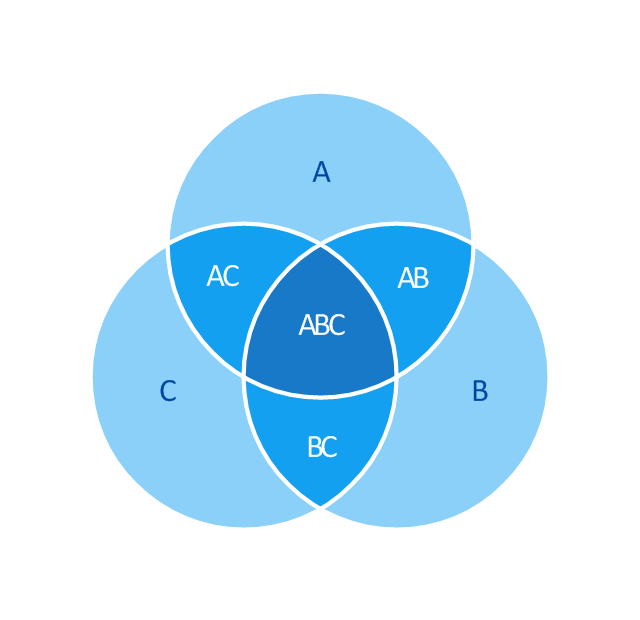
\includegraphics[scale=0.4]{ven.png}
        \caption{Diagrama de Venn}
    \end{figure}
    Sin pérdida de generalidad, definiendo los eventos $E_1 = A \cup B \cup C^c = ABC$,
    $E_2 = A \cup B^c \cup C = AB^cC$ y $E_3 = A^c \cup B \cup C = A^cBC$, cada uno de ellos
    solo ocurren dos de $A,B,C$. Cada evento definida previamente no tiene intersecciones,
    \textit{id est}, son disjuntos, entonces podemos verlos como:
    \begin{align*}
        &P(E_1) = P(AB) - P(ABC)\\
        &P(E_2) = P(AC) - P(ABC)\\
        &P(E_3) = P(BC) - P(ABC)
    \end{align*}
    Sea el evento $E := \{ \text{Solamente ocurran dos de $A,B,C$}\}$, ergo su probabilidad es:
    \begin{align*}
        P(E) 
            &= P(AB) - P(ABC) + P(AC) - P(ABC) + P(BC) - P(ABC)\\
            &= P(AB) + P(AC) + P(BC) - 3P(ABC)
    \end{align*}
\end{proof}
\item Prueba que $P(A_i) = 1$ para toda $i \geq 1$ entonces $P(\bigcap_{i=0}^{\infty} A_i) = 1$.

\textit{Hint}: Usa la Desigualdad de Boole

\sol \begin{proof}
    Recordando la desigualdad de Boole que es:
    \[
        P(\bigcup_{i=1}^{\infty} A_i) \leq \sum_{i=1}^{\infty} P(A_i)
    \]
\begin{align*}
    P(\bigcap_{i=0}^{\infty} A_i)
        &= 1 - (P(\bigcap_{i=1}^{\infty} A_i)^c) && \text{(Def. complemento)}\\
        &= 1 - P(\bigcup_{i=1}^{\infty} A_i^c) && \text{(De Morgan)}\\
        &\geq 1 - \sum_{i=1}^{\infty} P(A_i^c) && \text{(Desigualdad de Boole)}\\
        &\geq 1 - \sum_{i=1}^{\infty} (1 - P(A_i)) && \text{(Def. complemento)}\\
        &\geq 1 - \sum_{i=1}^{\infty} (1 - 1) && \text{(Por hipótesis)}\\
        &\geq 1 - \sum_{i=1}^{\infty} 0 && \text{(Aritmética)}\\
        &= 1
\end{align*}
\end{proof}

\item Sean $A,B \in S$ dos eventos. Decimos que: $A \sim B$ si $P(A \triangle B) = 0$.
Prueba que ($\sim$) es de equivalencia.

\sol
\begin{proof}
    Recordando las propiedades que debe de cumplir para que sea una relación de equivalencia.
    \begin{itemize}
    \item Reflexiva
    
    Por demostrar que $P(A \triangle A) = 0$. Por definición de diferencia simétrica tenemos que
    $P(A \triangle B) = P(A \setminus B) + P(B \setminus A)$ pero tenemos que
    $P(A \setminus A) + P(A \setminus A) = 0$, entonces cumple con ser reflexiva.
    
    Así $P(AB^c) = P(BA^c)$, por otro lado se tiene 

    \item Simétrica
    
    Por conmutatividad de definición de diferencia simetrica que es:
    \begin{align*}
        P(A \triangle B) 
            &= P(A \setminus B) + P(B \setminus A)\\
            &= P(B \setminus A) + P(A \setminus B)\\
            &= P(B \triangle A)
    \end{align*}

    \item  Transitiva
    
    TODO
    \end{itemize}
\end{proof}

\item Prueba el principio de inclusión-exclusión.
\[
    P(\bigcup_{i=1}^{n} A_i) = \sum_{i=1}^{n} P(A_i) - \sum_{1 \leq i < j \leq n } P(A_i \cap A_j)
    + \ldots + (-1)^{n+1} P(A_1 \cap \ldots \cap A_n) \tag{$\heartsuit$}
\]

\textit{Hint: Ver libro [DeGroot]-pp 48}

\sol (Por inducción)
\begin{proof}
\underline{Caso base:}
\begin{itemize}
    \item Para $n=1$. Trivial.
    \item Para $n=2$.
    
    Para esta prueba se utilizara el teorema que dice lo siguiente: Para cualesquiera dos eventos
    $A$ y $B$.
    \[
        P(A \cup B) = P(A) + P(B) - P(A \cup B) \tag{*}
    \]
    \begin{proof}
        \textbf{Partición de un conjunto:} Para cualesquiera dos conjuntos $A$ y $B$, $A \cap B$
        y $A \cap B^c$ son conjuntos disjuntos y $A = (A \cap B) \cup (A \cap B^c)$. En adición,
        $B$ y $A \cap B^c$ son disjuntos y $A \cup B = B \cup (A \cap B^c)$.


        Sabiendo eso, se tiene:
        $$A \cup B = B \cup (A \cap B^c)$$

        Como los dos eventos de la derecha son dusjuntos, se tiene que:
        \begin{align*}
            P(A \cup B) &=  P(B) - P(A \cap B^c) \tag{1}\\
                &= P(B) - P(A) - P(A \cap B) \tag{2}
        \end{align*}
        Pero en $(1)$ se sustiyuye $P(A \cap B^c)$ por $P(A) - P(A \cap B)$ en $(2)$porque hay un
        teorema que dice que sean dos eventos $A$ y $B$ se cumple que:
        $$P(A \cap B^c) = P(A) - P(A \cap B)$$
    \end{proof}
    Teniendo la igualdad del teorema previo demostrado, se tiene que 
    $P(A \cup B) = P(A) + P(B) - P(A \cup B)$.
\end{itemize}

\underline{Hipótesis de inducción:} Existe $m$ tal que es verdadero para toda $n \leq m$.

\underline{Paso inductivo:} Para $n=m+1$.

Sean $A_1, \ldots, A_{m+1}$ eventos. Definimos $A = \bigcup_{i=1}^{m} A_i$ y $B = A_{m+1}$ y usando
el teorema previo $(*)$, podemos decir que:
\begin{equation}
    P(\bigcup_{i=1}^{n} A_i) = P(A \cup B) = P(A) + P(B) - P(A \cup B) \tag{3}
\end{equation}

Se ha asumido que $P(A)$ es igual a $(\heartsuit)$ con $n=m$. Se necesita mostrar que cuando sumamos
$P(A)$ a $P(B) - P(A \cap B)$ se obtiene $(\heartsuit)$ con $n=m+1$. La diferencia entre
$(\heartsuit)$ con $n=m+1$ y $P(A)$ son todos los términos en que cada uno de los índices 
$(i,j,k,\ldots)$ son iguales a $m+1$. Esos términos son los siguientes
\begin{equation}
    P(A_{m+1}) - \sum_{i=1}^{m} P(A_i \cap A_{m+1}) + \sum_{i < j} P(A_i \cap A_j \cap A_{m+1}) +
    \ldots + (-1)^{m+2} P(A_1 \cap A_2 \cap \cdots \cap A_m \cap A_{m+1}) \tag{4}
\end{equation}

El primer término en $(4)$ es $P(B) = P(A_{m+1})$. Todo lo que queda es mostrar que $-P(A \cup B)$
es igual a todos, pero el primer término en $(4)$.

Usando la generalización de la propiedad distributiva, para escribir que:
\[
    A \cap B = (\bigcup_{i=1}^m A_i) \cap A_{m+1} = \bigcup_{i=1}^{m} (A_i \cap A_{m+1}) \tag{5}
\]

La unión en $(5)$ contiene $m$ eventos, y por tanto podemos aplicar $(\heartsuit)$ con $n=m$ y cada
$A_i$ reemplazada por $A_i \cap A_{m+1}$. El resultado es que $-P(A \cap B)$ es igual a todos,
excepto el primer término en $(4)$.
\end{proof}


\item Leer y desarrollar el problema ``(6a)- \textbf{Probabilidad y una Paradoja''
[Ross-8th. Ed]- pp 46-48}

\sol Suponemos que tenemos una urna infinitamente grande y una colección infinita de pelotas
etiquetadas. Se considera el experimento como sigue: a un minuto de las 12 p.m. las pelotas
numeradas del 1 al 10 son puestas en la urna y la pelota número 10 es recogida. (Suponer que la
acción de recoger una pelota no toma tiempo). A $\frac{1}{2}$ minuto para laras las 12 p.m. las 
pelotas de la 11 a las 20 son puestas en la urna y la pelota número 20 es recogida de la urna.
A $\frac{1}{4}$ minuto para laras las 12 p.m. las  pelotas de la 21 a la 30 son puestas en la urna y
la pelota número 30 es recogida de la urna. Y así sucesivamente. La pregunta aquí es ¿cuántas
pelotas hay en la urna a las 12 p.m.?

La resupuesta es que hay un número infinito de pelotas en la urna a las 12 p.m., esto es porque toda
aquella pelota que no es de la forma $10n$, con $n \geq 1$ será puesta en la urna. Por tanto el 
problema está resuelto a como está descrito.

Sin embargo, ahora se cambiará el experimento y se supondrá que a 1 minuto de las 12 p.m. las
pelotas numeradas del 1 al 10 serán puestas en la urna y se removerá la pelota número 1. A
$\frac{1}{2}$ de las 12 p.m. las pelotas númeras del 11 al 20 serán puestas en la urna y será
removida la pelota número 2 y así sucesivamente. Para este nuevo experimento, se pregunta
¿Cuántas pelotas hay en la urna a las 12 p.m.?

Sorprendentemente a las 12 p.m. la urna está vacía. Considerando cualquier pelota, digamos, la
pelota $n$. En un punto antes de las 12 p.m. (en particular a $(\frac{1}{2})^{n-1}$ antes de las
12 p.m.) pudo haber sido removida de la urna. Por tanto, para cada $n$, la pelota $n$ no está en la
urna a las 12 p.m., por lo tanto, la urna tuvo que haber estado vacía a este tiempo.

Entonces \textbf{vemos que la manera en que las pelotas son removidas hace la diferencia}.
Supongamos que cualquier pelota puede ser removida, que la pelota sea aleatoriamente seleccionada
y sacada de la urna, y así sucesivamente. En este caso la preguntas es ¿Cuántas preguntas hay en
la urna a las 12 p.m.?

Lo que queremos mostrar es que con probabilidad 1, la urna está vacía a las 12 p.m. Consideremos
primero la pelota número 1. Definamos $E_n$ al evento que la pelota número 1 siga estando en la urna
después de $n$ que se hayan hecho $n$ extracciones de la urna. Claramente
$$P(E_n) = \frac{9 \cdot 18 \cdot 27 \cdots (9n)}{10 \cdot 19 \cdot 19 \cdots (9n+1)}$$

Ahora, el evento que la pelota número 1 esté en la urna a las 12 p.m. es el evento
$\cap_{n=1}^{\infty} E_n$. Porque los eventos $E_n$, $n \geq 1$, son eventos decrecientes, que es
$P(E) = P\{ \text{La pelota número 1 está en la urna a las 12 p.m.} \}$.
\[
    P(E) = \bigcap_{n=1}^{\infty} E_n = \lim_{n \to \infty} P(E_n) =
    \prod_{n=1}^{\infty} (\frac{9n}{9n+1})
\]
Y lo que queremos mostrar es que $\prod_{n=1}^{\infty} (\frac{9n}{9n+1}) = 0$.

Dado que:
\[
    \prod_{n=1}^{\infty} (\frac{9n}{9n+1}) = [\prod_{n=1}^{\infty} (\frac{9n+1}{9n})]^{-1}
\]
Es equivalente a mostrar que:
\[
    \prod_{n=1}^{\infty} (1 + \frac{1}{9n}) = \infty
\]
Ahora, para toda $m \geq 1$,
\begin{align*}
    \prod_{n=1}^{\infty} (1 + \frac{1}{9n})
        &= \prod_{n=1}^{m} (1 + \frac{1}{9n})\\
        &= (1 + \frac{1}{9}) (1 + \frac{1}{18}) (1 + \frac{1}{27}) \cdots (1 + \frac{1}{9m})\\
        &> \frac{1}{9} + \frac{1}{18} + \frac{1}{27} + \ldots + \frac{1}{9m}\\
        &= \frac{1}{9} \sum_{i=1}^{m} \frac{1}{i}
\end{align*}
Por tanto, haciendo $m \to \infty$ y usando el hecho de que $\sum_{i=1}^{m} \frac{1}{i} = \infty$
genera:
$$\prod_{n=1}^{\infty} (1 + \frac{1}{9n}) = \infty$$
Por lo tanto, haciendo que $F_i$ denote el evento que la pelota número $i$ esté en la urna a las
12 p.m., hemos mostrado que $P(F_1)= 0$. Similarmente, podemos mostrar que $P(F_i)=1$ para
toda $i$.

Por lo tanto, la probabiliad de que la urna no esté vacía a las 12 p.m.,
$P(\bigcup_{1}^{\infty} F_i)$, satisface que:
\[
    P(\bigcup_{1}^{\infty} F_i) \leq \sum_{1}^{\infty} P(F_i) = 0
\]
Por lo tanto, con probabilidad 1, la urna va a estras vacía a las 12 p.m.


\item Dado un conjunto $S$. Si para alguna $k \geq 1$. Se tiene que $S_1, S_2, \ldots, S_k$ son
subconjuntos mutuamente excluyetes de $S$ talque $\bigcup_{i=1}^{k} S_i = S$ entonces decimos
que la clase $\{ S_1, S_2, \ldots, S_k \}$ es una \textbf{Partición} de $S$. Sea $T_n$ el número
de diferentes particiones de $\{ 1, 2, \ldots , n \}$. Así por ejemplo tenemos que
$T_1 = 1$ (La única partición posible es $S_1 = \{ 1 \}$ y $T_2 = 2$ (Las dos particiones
posibles de un conjunto de dos elementos son $\{ \{ 1, 2 \}, \{ \{ 1 \}, \{ 2 \} \} \}$).

\begin{itemize}
    \item Exhibe las particiones y muestra que $T_3 = 5$, $T_4 = 15$.
    
    \sol
    \begin{itemize}
        \item $T_3 = 5$
        
        Primero podemos tener a los subconjuntos $\{1\}$, $\{2\}$ y $\{3\}$.
        
        Después, podemos tener un subconjunto con un subconjunto de un elemento y otro subconjunto
        con otro de 2 elementos. Quedando tres formas de hacerlos como:
        \begin{align*}
            \{1\}, \{2, 3\}\\
            \{2\}, \{1, 3\}\\
            \{3\}, \{1, 2\}
        \end{align*}

        Al final, tenemos un conjunto con tres elemntos en un subconjunto el cual es $\{1,2,3\}$.

        Por tanto, hay 5 formas de particionar al conjunto.

        \item $T_4 = 15$
        \begin{align*}
            &\{\{1, 2, 3, 4\}\}\\
            &\{\{1, 2, 3\}, \{4\}\}\\
            &\{\{1, 2, 4\}, \{3\}\}\\
            &\{\{1, 2\}, \{3, 4\}\}\\
            &\{\{1, 3, 4\}, \{2\}\}\\
            &\{\{1, 3\}, \{2, 4\}\}\\
            &\{\{1, 4\}, \{2, 3\}\}\\
            &\{\{1\}, \{2, 3, 4\}\}\\
            &\{\{1, 2\}, \{3\}, \{4\}\}\\
            &\{\{1, 3\}, \{2\}, \{4\}\}\\
            &\{\{1\}, \{2, 3\}, \{4\}\}\\
            &\{\{1, 4\}, \{2\}, \{3\}\}\\
            &\{\{1\}, \{2, 4\}, \{3\}\}\\
            &\{\{1\}, \{2\}, \{3, 4\}\}\\
            &\{\{1\}, \{2\}, \{3\}, \{4\}\}
        \end{align*}

    \end{itemize}

    \item Demuestra que
    \[
        T_{n+1} = 1 + \sum_{k=1}^{n} \binom{n}{k} T_k
    \]
    Usar este resultado para culcular $T_{10}$

    A esta serie de números $T_i's$ se les conoces como \textbf{Números de Bell}.

    \begin{proof}
        \[
            T_{n+1} = \sum_{i=1}^{n} \binom{n}{i} T_{n-i} =1 + \sum_{i=0}^{n-1} \binom{n}{i} T_{n-i} =
            1 + \sum_{k=1}^{n} \binom{n}{k} T_{n-k}
        \]
    \end{proof}

    Para calcular el $T_{10}$ se procedió a hacer un programa en \textit{Python} haciendo uso
    de programación dinámica, con la siguiente función.

    \begin{lstlisting}[language=Python]
    def bell_bumber(n): 
    
        bell = [[0 for i in range(n+1)] for j in range(n+1)] 
        bell[0][0] = 1
        for i in range(1, n+1): 
    
            bell[i][0] = bell[i-1][i-1] 
    
            for j in range(1, i+1): 
                bell[i][j] = bell[i-1][j-1] + bell[i][j-1] 
    
        return bell[n][0] 
    
    print(bell_bumber(10)) 
    \end{lstlisting}

    Dando como resultado $T_{10} = 115975$.

    \item Exhibe las primeras 5 filas del \textbf{Triángulo de Bell}.
    
    \sol
\begin{verbatim*}
1
1 2
2 3 5
5 7 10 15
15 20 27 37 52
\end{verbatim*}

    \item Realiza una breve semblanza de dos de los mas grandes matemáticos del Siglo XX.
    \textbf{Srinivasa Ramanujuan} y \textbf{Eric Bell}.

    \sol

    Srinivasa Ramunajam, matemático indio (1987 – 1920). Fue un matemático de excepción. Durante su
    breve vida llegó a publicar más de 3000 resultados entre demostraciones e identidades. Decía que
    su inspiración era la visita de la diosa Namagiri durante sueños. La mayor incógnita acerca de
    este hombre era el mismo. Su falta de educación formal y sus múltiples carencias económicas y
    todo tipo no fueron impedimento para que este hombre nacido en la india llegara a transformarse
    sólo de manera autodidacta en el más grande matemático de su país.
    Ramanujan era un apasionado de las secuencias y las series infinitas, las que aparecen
    desparramadas en todas sus notas. Junto con Hardy, emprendió el estudio de una secuencia de
    extrema importancia:

    1, 2, 3, 5, 7, 11, 15, 22, 30, 42, 56, 77, 101, 135, 176, 231, 297, 385, 490, 627, 792, 1002,
    1255, 1575, 1958, 2436, 3010, 3718, \dots

    En ella, el término que aparece en la posición corresponde al número de maneras de escribir como
    suma de enteros positivos. En otras palabras, es la cantidad de maneras distintas de ``partir''
    el número en piezas aditivas, sin distinguir particiones en las que aparecen los mismos sumandos
    pero dispuestos en distinto orden.

    Ramanujan fue galardonado con una licenciatura en Ciencias (este grado fue más tarde renombrado
    PhD) en marzo de 1916 por su trabajo de investigación en números altamente compuestos, la
    primera parte de la cual fue publicada como un documento en las Actas de la London Mathematical
    Society.

    El artículo tenía más de 50 páginas con la demostración de diferentes propiedades de tales
    números. Hardy comentó que este fue uno de los artículos más inusuales surgidos en la
    investigación matemática de esa época y que Ramanujan mostró un extraordinario ingenio en su
    manejo.


    Eric Temple Bell nació un 7 de febrero de 1883 en  Escocia. Tras una fructífera y extensa
    carrera profesional muere a la de edad de 77 años el día 21 de diciembre de 1960 en Watsonville
    pueblo americano del estado de California al que se mudó años atrás. Se le conoce sobretodo por
    ser un brillante matemático y autor de novelas de ciencia ficción. Como ya se ha comentado nació
    en Escocia pero vivió la mayor parte de su vida en los EE.UU. 

    Sus principales logros se basan en las investigaciones sobre la teoría de los números. Intentó
    también pero sin éxito explicar el llamado cálculo tradicional umbral también conocido como el
    ``método simbólico'' de Blissard. Se le considera que fue él quien postuló, y por eso recibe su
    nombre, el método de la Campana de los polinomios y números de Bell. En 1924 se le concedió el
    prestigioso Premio Bôcher Memorial por su exitosa labor en el análisis matemático.

    Su mayor éxito fue un libro titulado ``Los hombres de las matemáticas'' que inspiró a muchas
    personas a interesarse por las matemáticas, aunque a posteriori algunos historiadores han
    cuestionado la precisión a la hora de escribir de Bell. Otro de sus últimos libros fue
    ``El desarrollo de las matemáticas'' que aunque ha sido menos famoso se considera que tiene
    muchos menos puntos débiles en su precisión.

\end{itemize}


\end{enumerate}


%%%%%%%%%%%%%%%%%%%%%%%%%%%%%%%%%%%%%%%%%%%%%%%%%%%%%%%%%%%%%%%%%%%%%%%%%%%%%%%%%%%%%%%%%


%%%%%%%%%%%%%%%%%%%%%%%%%%%%%%%%%%%%%%%%%%%%%%%%%%%%%%%%%%%%%%%%%%%%%%%%%%%%%%%%%%%%%%%%%

%%%%%%%%%%%%%%%%%%%%%%%%%%%%%%%%%%%%%%%%%%%%%%%%%%%%%%%%%%%%%%%%%%%%%%%%%%%%%%%%%%%%%%%%%

\end{document}